\documentclass[tikz,border=10pt]{standalone}
\usepackage{tikz}

\begin{document}

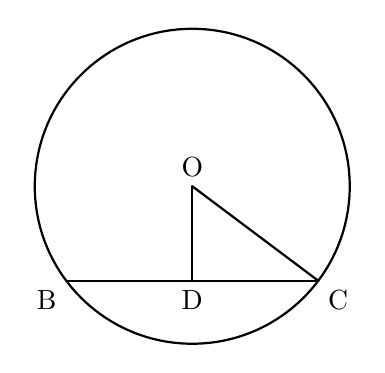
\begin{tikzpicture}[scale=1, line cap=round, line join=round]

% Define coordinates
% Center of the circle
\coordinate (O) at (0,0);

% Define points B and C on the circle
% We'll place the chord BC in the lower part of the circle
\coordinate (B) at (-1.6, -1.2);
\coordinate (C) at (1.6, -1.2);

% Define point D as the foot of the perpendicular from O to BC
\coordinate (D) at (0, -1.2);

% Calculate radius based on point C
% Radius r = sqrt(1.6^2 + 1.2^2) = 2
\draw[thick] (O) circle (2);

% Draw the line segments
\draw[thick] (B) -- (C);   % Chord BC
\draw[thick] (O) -- (D);   % Segment OD (perpendicular to chord)
\draw[thick] (O) -- (C);   % Radius OC

% Label the points
\node[above] at (O) {O};
\node[below left] at (B) {B};
\node[below] at (D) {D};
\node[below right] at (C) {C};

\end{tikzpicture}

\end{document}
